\documentclass[a4paper,12pt]{book}

% Paquetes necesarios
\usepackage[utf8]{inputenc}   % Codificación de caracteres
\usepackage[spanish]{babel}   % Idioma español
\usepackage[T1]{fontenc}      % Codificación de fuentes
\usepackage{amsmath, amssymb} % Símbolos matemáticos
\usepackage{graphicx}         % Inclusión de gráficos
\usepackage{cite}             % Gestión de citas
\usepackage{hyperref}         % Enlaces y referencias
\usepackage{geometry}         % Configuración de márgenes
\usepackage{fancyhdr}         % Encabezados y pies de página
\usepackage{titlesec}         % Formato de títulos
\usepackage{booktabs}         % Tablas profesionales
\usepackage{caption}          % Personalización de leyendas
\usepackage{enumitem}         % Personalización de listas
\usepackage{float}
\usepackage{tcolorbox}
\usepackage[table]{xcolor} % Paquete para colores en tablas
\usepackage{colortbl}       % Complemento para colorear celdas específicas
\usepackage{multirow}       % Combinar celdas en tablas
\usepackage{makecell}       % Combinar celdas en tablas
\usepackage{enumitem}
\usepackage{amsmath}
\usepackage{eurosym}
\usepackage{tikz}
\usepackage{listings}
\usepackage{color}
\usepackage{float}
\usepackage{pdfpages}
\usepackage{fancyhdr}
\usepackage{lastpage}
\usepackage{hyperref}
\usepackage{titlesec}
\usepackage{aligned-overset}
\usepackage{amsmath}
\usepackage{amssymb}
\usepackage{nicefrac}
\usepackage{graphicx}
\usepackage{subcaption}
\usepackage{pgfplots}

% Configuración de márgenes
\geometry{left=3cm, right=3cm, top=2.5cm, bottom=2.5cm}

% Configuración de encabezados y pies de página
% \setlength{\headheight}{14.49998pt}
\pagestyle{fancy}
\fancyhf{}
\fancyhead[L]{Universidad de Granada}
\fancyhead[L]{\nouppercase{ \leftmark}}

% \fancyhead[C]{Escuela Técnica Superior de Ingenierías Informática}

%\fancyhead[L]{Universidad de Granada}
\fancyhead[L]{\nouppercase{\chaptername \thechapter. \leftmark}}
\fancyhead[R]{Ingeniería de Servidores}
\fancyfoot[L]{\rule[0pt]{\textwidth}{0.2pt}\\Ismael Sallami Moreno}
\fancyfoot[C]{\rule[0pt]{\textwidth}{0.2pt}\\\thepage}
\fancyfoot[R]{\rule[0pt]{\textwidth}{0.2pt}\\\today}


\renewcommand{\sectionmark}[1]{\markboth{#1}{}} % Configura \leftmark para que solo muestre la sección

% Formato de títulos
\titleformat{\section}{\large\bfseries}{\thesection.}{0.5em}{}
\titleformat{\subsection}{\normalsize\bfseries}{\thesubsection.}{0.5em}{}

% Datos del documento
\title{\textbf{Temario Ingeniería de Servidores}}
\author{
    Ismael Sallami Moreno \\
    \texttt{ism350zsallami@correo.ugr.es}
}
\date{
    \vspace{1cm}
    \begin{tabular}{rl}
        \textbf{Asignatura:} & Ingeniería de Servidores \\
        \textbf{Tema:} & Teoría \\
        \textbf{Fecha:} & \today
    \end{tabular}
}

\begin{document}

% Portada
\begin{titlepage}
    \begin{center}
        % \vspace*{1cm}
        
        % \Huge
        % \textbf{Práctica Contabilidad Financiera II}
        \Huge \textbf{Temario Ingeniería de Servidores} 
        % \vspace{0.5cm}
        % \LARGE
        % \textbf{Ismael Sallami Moreno}\\
        % \LARGE
        % \texttt{ism350zsallami@correo.ugr.es}
        % \LARGE
        % \url{https://github.com/Ismael-Sallami}
        
        % \vfill
        
        % \Large
        % \textbf{Universidad de Granada}
        
        \vspace{0.8cm}
        
        \begin{tikzpicture}[remember picture, overlay]
            \node[opacity=0.2] at (current page.center) {
\includegraphics[width=\paperwidth,height=\paperheight]{portada.jpg}};
            \node[align=center] at (current page.center) {
                
                \vspace{0.5cm}
                \LARGE \textbf{Ismael Sallami Moreno} \\
                \LARGE \texttt{ism350zsallami@correo.ugr.es} \\
                \LARGE \url{https://ismael-sallami.github.io/} \\
                \LARGE \url{https://elblogdeismael.github.io/} \\
                \vspace{2cm}
                \Large \textbf{Universidad de Granada} \\
                \vspace{0.8cm}
                % \Large \textbf{2025}
            };
        \end{tikzpicture}
        \vfill
        
        \Large
        \textbf{2025}
        
    \end{center}
\end{titlepage}
\newpage


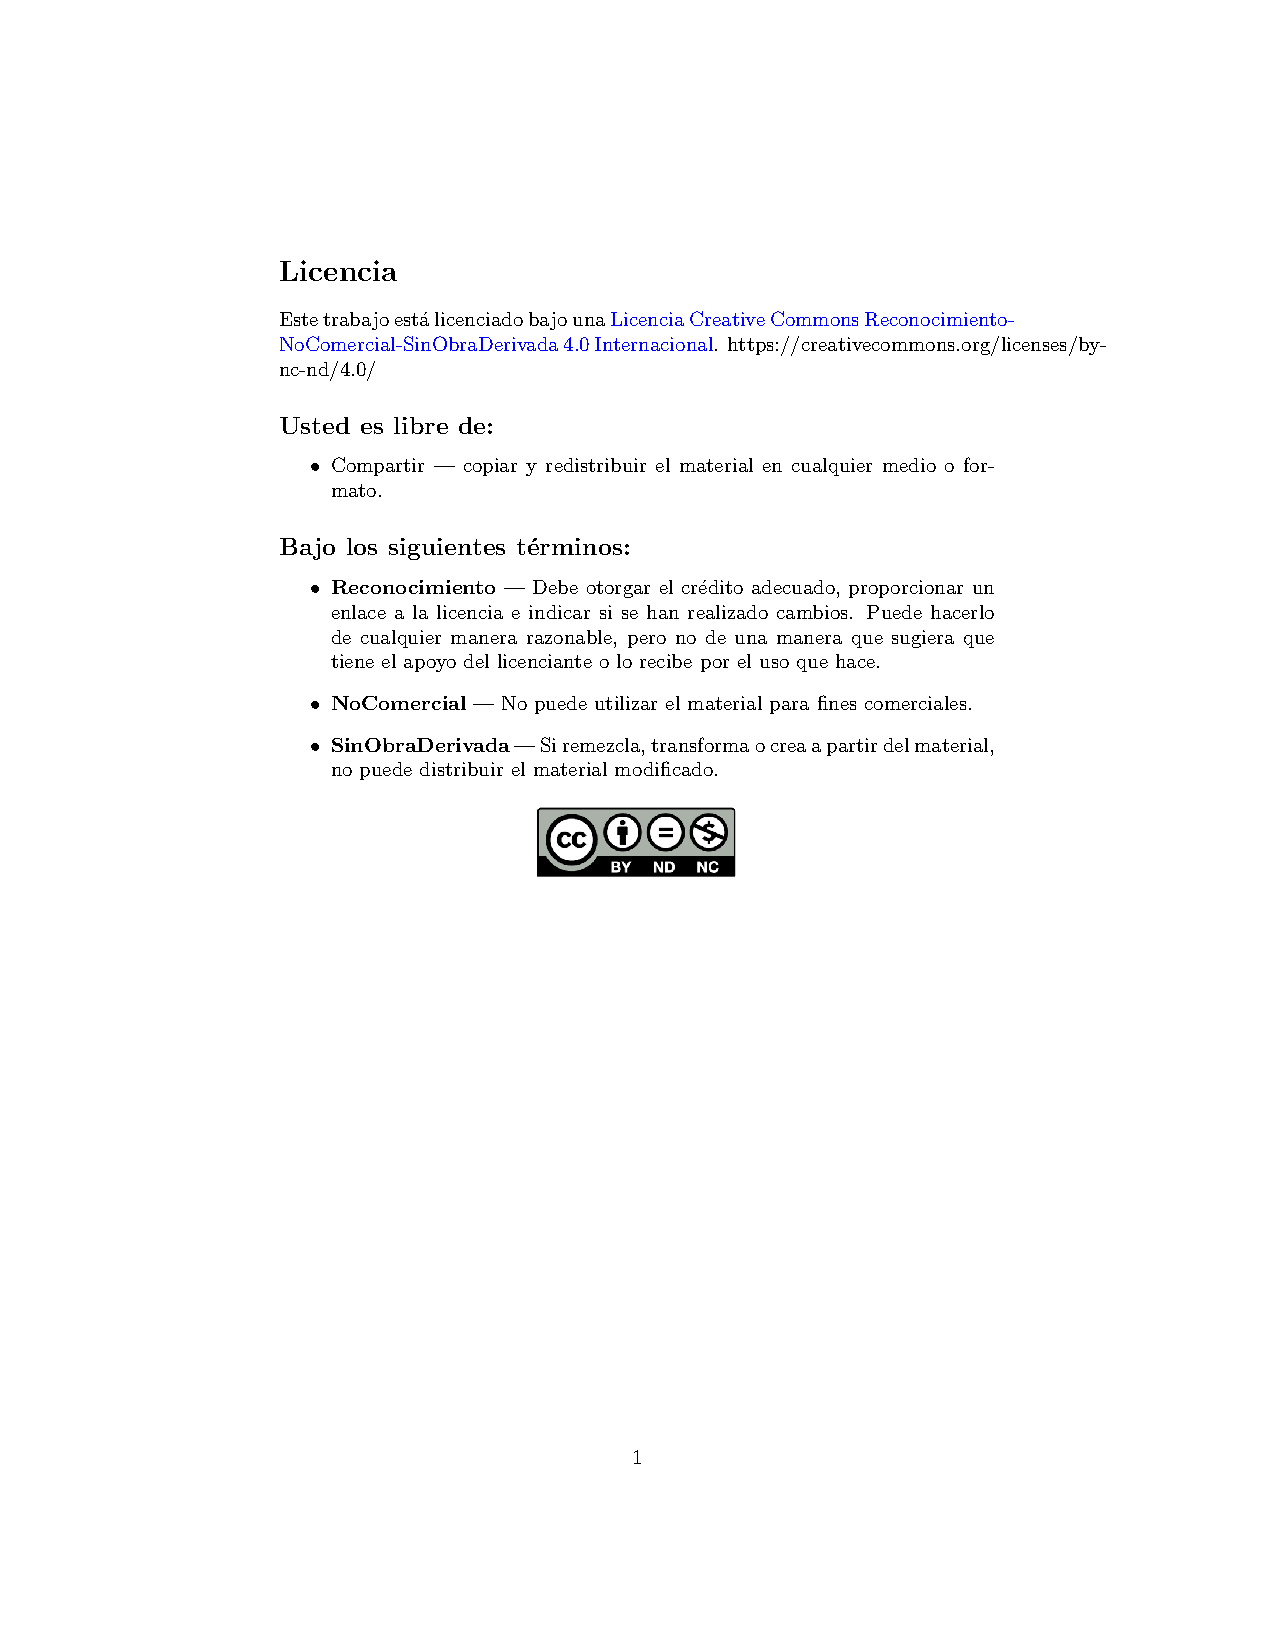
\includepdf[pages=-]{../../../../licencia.pdf}
% Tabla de contenidos
\tableofcontents
\newpage

\chapter{Introducción a la Ingeniería de Servidores}
% \section{Apuntes de Clase}
% \section{Introducción}
Este es un documento de prueba en \LaTeX. Aquí puedes escribir el contenido de tu primer capítulo.

\section{Definiciones Básicas}
\subsection{Definición 1}
Una definición básica para comenzar:
\[
E = mc^2
\]
donde $E$ es la energía, $m$ es la masa y $c$ es la velocidad de la luz.

\subsection{Definición 2}
Otra definición importante:
\[
a^2 + b^2 = c^2
\]
que corresponde al teorema de Pitágoras.

\section{Conclusión}
Este es un ejemplo básico de cómo estructurar un capítulo en \LaTeX. Puedes expandirlo según tus necesidades.

\section{Ejercicios Tema 1}
%\includepdf[pages=-,pagecommand={\thispagestyle{fancy}}]{Capitulos/Ejercicios_ISE_T1.pdf}
\input{Capitulos/EjerciciosT1.tex}

% \section{Diapositivas Tema 1}
% 
\includepdf[pages=-,pagecommand={\thispagestyle{fancy}}]{Capitulos/Tema1.pdf}


\chapter{Componentes Hardware de un Servidor}
% \section{Apuntes de Clase}
% \section{Ejercicios}

\subsection*{Ejercicio 1 }

\begin{enumerate}
    \item En el Boletín de Deuda Pública del día 23 de marzo de 2012, en su sección de operaciones de compraventa simple al contado sobre Deuda del Estado, podemos encontrar la siguiente información:
    
    \begin{table}[h!]
        \centering
        \begin{tabular}{|c|c|c|c|c|}
            \hline
            \textbf{EMISIÓN} & \textbf{Cupón} & \textbf{Amortización} & \textbf{Precio medio ex cupón} & \textbf{TIR} \\
            \hline
            ES00000123B9 O EST & 5.50 & 30.04.21 & 101,105 & 5,34 \\
            \hline
        \end{tabular}
    \end{table}

    \begin{tikzpicture}
        % Línea de tiempo
         \draw[-] (0,0) -- (12,0) node[right] {Tiempo};
    
        % Emisión inicial
        \draw[-{Latex}] (0,0) -- (0,-1) node[below right, yshift=-0.5cm, xshift=-1.5cm, align=center, text width=3cm] {30/04/12\\Emisión\\1000};
    
        % Pagos periódicos
        \draw[-{Latex}] (2,0) -- (2,1) node[above, yshift=0.4cm, align=center, text width=3cm] {30/04/14};
        \draw[-{Latex}] (4,0) -- (4,1) node[above, yshift=0.4cm, align=center, text width=3cm] {30/04/15};
        \draw[-{Latex}] (6,0) -- (6,1) node[above, yshift=0.4cm, align=center, text width=3cm] {...};
        \draw[-{Latex}] (12,0) -- (12,1) node[above, yshift=0.4cm, align=center, text width=3cm] {30/04/21\\};
    
        % % Emisión final
        % \draw[-{Latex}] (11.8,0) -- (11.8,-1) node[below right, yshift=-0.5cm, xshift=-1.5cm, align=center, text width=3cm] {30/04/21\\};
    
    
    
        % Conversión
        % \draw[-{Latex},red] (3,0) -- (3,-1) node[below left, yshift=-0.8cm, xshift=-0.3cm, align=center, text width=3cm] {31/3/06\\Conversión};
    
        % % Venta
        % \draw[-{Latex},blue] (3.5,0) -- (3.5,1) node[above, yshift=0.8cm, align=center, text width=3cm] {30/4/06\\Venta};
    
        % % Amortización final
        % \draw[-{Latex}] (10,0) -- (10,-1) node[below right, yshift=-0.8cm, xshift=0.3cm, align=center, text width=3cm] {31/12/09\\Amortización\\1020};
    
    \end{tikzpicture}
    
    \begin{enumerate}
        \item[a)] Si se supone que se ha comprado esta obligación por el precio medio, ¿Cuánto se ha pagado por ella? \textbf{Sol: 1.060,34€}
        
        \begin{itemize}
            \item Del 30/04/11 al 23/03/12 hay 328 días.
            \item Del 23/03/12 al 30/04/12 hay 38 días.
            \item El total es de 366 días.
        \end{itemize}

        \begin{equation*}
            P_{\text{total}} = 101,105 \times 1000 + \frac{55}{366} \times 328 = 1.060,34
        \end{equation*}
        \item[b)] Plantea la ecuación que verifica la TIR con la que se está contratando esta obligación y calcula su valor. \textbf{Sol: 5,34\%}
        \begin{equation*}
            1060,34 = \left[55 \times a_{10,TIR}+\frac{1000}{(1+TIR)^{10}}\right]\times(1+TIR)^{\frac{328}{366}}
        \end{equation*}
    \end{enumerate}
\end{enumerate}

\textit{Debemos de hacer ciertas suposiciones como es el caso de que al amortizarse en 30.04.21, y estamos a 23.03.12, el comienzo de la vida de la obligación es el 30.04.12.}
\\\\

% \begin{tikzpicture}
%     % Línea de tiempo
%      \draw[-] (0,0) -- (12,0) node[right] {Tiempo};

%     % Emisión inicial
%     \draw[-{Latex}] (0,0) -- (0,-1) node[below right, yshift=-0.5cm, xshift=-1.5cm, align=center, text width=3cm] {30/04/12\\Emisión\\1000};

%     % Pagos periódicos
%     \draw[-{Latex}] (2,0) -- (2,1) node[above, yshift=0.4cm, align=center, text width=3cm] {30/04/14};
%     \draw[-{Latex}] (4,0) -- (4,1) node[above, yshift=0.4cm, align=center, text width=3cm] {30/04/15};
%     \draw[-{Latex}] (6,0) -- (6,1) node[above, yshift=0.4cm, align=center, text width=3cm] {...};
%     \draw[-{Latex}] (12,0) -- (12,1) node[above, yshift=0.4cm, align=center, text width=3cm] {30/04/21\\};

%     % % Emisión final
%     % \draw[-{Latex}] (11.8,0) -- (11.8,-1) node[below right, yshift=-0.5cm, xshift=-1.5cm, align=center, text width=3cm] {30/04/21\\};



%     % Conversión
%     % \draw[-{Latex},red] (3,0) -- (3,-1) node[below left, yshift=-0.8cm, xshift=-0.3cm, align=center, text width=3cm] {31/3/06\\Conversión};

%     % % Venta
%     % \draw[-{Latex},blue] (3.5,0) -- (3.5,1) node[above, yshift=0.8cm, align=center, text width=3cm] {30/4/06\\Venta};

%     % % Amortización final
%     % \draw[-{Latex}] (10,0) -- (10,-1) node[below right, yshift=-0.8cm, xshift=0.3cm, align=center, text width=3cm] {31/12/09\\Amortización\\1020};

% \end{tikzpicture}

% \begin{itemize}
%     \item Del 30/04/11 al 23/03/12 hay 328 días.
%     \item Del 23/03/12 al 30/04/12 hay 38 días.
%     \item El total es de 366 días.
% \end{itemize}
% Así que calculando el precio total con la fórmula del precio excupón tenemos que:
% \begin{itemize}
%     \item [a)] \begin{equation*}
%         P_{\text{total}} = 101,105 \times 1000 + \frac{55}{366} \times 328 = 1.060,34
%     \end{equation*}


%     \item [b)] \begin{equation*}
%         1060,34 = \left[55 \times a_{10,TIR}+\frac{1000}{(1+TIR)^{10}}\right]\times(1+TIR)^{\frac{328}{366}}
%     \end{equation*}
% \end{itemize}


\subsection*{Ejercicio 2}

\begin{enumerate}
    \item La sociedad ILIGRASA emitió, el 1 de enero de 2011, obligaciones con:
    \begin{itemize}
        \item Valor nominal de 3.000€.
        \item Cupón al 5\% nominal anual pagadero por semestres (30 de junio y 31 de diciembre de cada año).
        \item Vencimiento a 10 años.
    \end{itemize}
    Los títulos se emitieron a la par sin gastos para el suscriptor. Hoy, 21 de junio de 2013, estos títulos cotizan en el mercado secundario al 108\% excupón.

    \begin{enumerate}
        \item[a)] Plantea la ecuación que verifica la rentabilidad que el mercado exige hoy a estos títulos y calcula su valor. \textbf{Sol: 3,7997\%.}
        Como primer paso debemos de calcular el $C_s$, el cual nos queda $C_s = \frac{5\%}{2} \times 3000 = 75$\footnote{Se divide entre 2 porque el pago es semestral y me dan el tipo de interés anual.}. 

        A continuación, caculamos el precio total, el cual nos queda:
        \begin{equation*}
            {P_T}_{\textit{21.06.13}} = 108\% \times 3000 + \frac{75}{181} \times 172 = 3311,27
        \end{equation*}

        Por lo que teniendo en cuenta que los días que han pasado desde el último pago son 172, podemos plantear la ecuación de la rentabilidad que el mercado exige hoy a estos títulos:

        \begin{equation*}
            3311,27 = \left[75 + a_{16,TIR_semestral} + \frac{3000}{(1+TIR)^{16}}\right] \times (1+TIR)^{\frac{172}{181}}
        \end{equation*}
        \item[b)] Si un inversor compró 15 títulos en la emisión y los vende hoy a través de un intermediario, cobrándole éste una comisión del 0,3\% sobre el valor efectivo de la venta, ¿qué rentabilidad efectiva ha obtenido con ellos? \textbf{Sol: 8,0361\%.}\\\\
        Se emitió a la par, por lo que es igual a el VN.
        El precio de venta es $ P_{venta} = 3311,27 -0,3 \times 3311,27 = 3301,34$

        La rentabilidad efectiva es:
        \begin{equation*}
            3000 = 75 \times a_{4,TIR} + \frac{3301,34}{1+TIR}^{\alpha}
        \end{equation*}

        Donde $\alpha$ es:
        \begin{align*}
            \alpha = \frac{4s+1ts = 172\text{días}+4s}{181}
        \end{align*}
        Donde denotamos s como semestre y ts como un trozo del simestre.
    \end{enumerate}
\end{enumerate}


\subsection*{Ejercicio 3}

El 1 de enero de 2011, cierta sociedad realizó una emisión de obligaciones con valor nominal unitario de 6.000€, cupón trimestral al 6\% nominal y vencimiento a 10 años. La emisión se realizó a la par e incluía una cláusula de rescate anticipado con un precio de rescate igual al 110\% del valor nominal de la obligación más el cupón corrido correspondiente. Hoy, 16 de abril de 2013, la rentabilidad que exige el mercado para estas obligaciones es del 4\% nominal.

Podemos representar la casuísitca de la siguiente manera:

\begin{tikzpicture}
    % Línea de tiempo
    \draw[-] (0,0) -- (12,0) node[right] {Tiempo};

    % Fechas
    \draw[-{Latex}] (0,0) -- (0,-1) node[below, yshift=-0.5cm, align=center, text width=3cm] {01/01/11\\Emisión};
    \draw[-{Latex}] (1,0) -- (1,-1) node[below, yshift=0cm, align=center, text width=3cm] {/12};
    \draw[-{Latex}] (2,0) -- (2,-1) node[below, yshift=0cm, align=center, text width=3cm] {/13};
    \draw[-{Latex}] (4,0) -- (4,-1) node[below, yshift=-0.5cm, align=center, text width=3cm] {1/04/13};
    \draw[-{Latex}] (6,0) -- (6,-1) node[below, yshift=-0.5cm, align=center, text width=3cm] {\textcolor{red}{16/04/13}};
    \draw[-{Latex}] (9.3,0) -- (9.3,-1) node[below, yshift=-0.5cm, align=center, text width=3cm] {/14};
    \draw[-{Latex}] (10,0) -- (10,-1) node[below, yshift=-0.5cm, align=center, text width=3cm] {...};
    \draw[-{Latex}] (8,0) -- (8,-1) node[below, yshift=-0.5cm, align=center, text width=3cm] {21/06/13};
    \draw[-{Latex}] (12,0) -- (12,-1) node[below, yshift=-0.5cm, align=center, text width=3cm] {30/04/21\\Vencimiento};
\end{tikzpicture}



\begin{enumerate}
    \item[a)] Calcula el precio de cotización de estas obligaciones hoy.
    
    \begin{align*}
        P_T = P_{\text{excupón}} + CC 
    \end{align*}

    \begin{center}
        \begin{tikzpicture}
            % Línea de tiempo
            \draw[-] (0,0) -- (12,0) node[right] {Tiempo};
    
            % Fechas
            \draw[-{Latex}] (0,0) -- (0,-1) node[below, yshift=-0.5cm, align=center, text width=3cm] {01/04/13};
            \draw[-{Latex}] (6,0) -- (6,-1) node[below, yshift=-0.5cm, align=center, text width=3cm] {16/04/13};
            \draw[-{Latex}] (12,0) -- (12,-1) node[below, yshift=-0.5cm, align=center, text width=3cm] {01/07/13};
    
            % Línea de días
            \draw[|-|] (0,-2.7) -- (6,-2.7) node[midway, below] {15 días};
            \draw[|-|] (0,-4) -- (12,-4) node[midway, below] {91 días};
        \end{tikzpicture}
    \end{center}

    \begin{align*}
        \text{Cupón} = \frac{6\%}{4} \times 6000 = 90 \\
        \text{CC}_{16/04/13} = \frac{90}{91} \times 15 = 14,84 \\
        n = 10 \times 4 - 9 (\text{ ya han pasado })= 31 \text{ trimestres } \\
        P_T = \left[63,3 \times a_{31,0'01} + \frac{6000}{1,01^{31}}\right] \times 1,01^{16/91} = 6807,42\\
        P_{\text{cotización = excupón}} = P_T - CC = 6807,42 - 14,84 = 6792,58
    \end{align*}

    Para saber la cotización $\rightarrow \frac{6792,58}{6000} \times 100 = 113,21\%$



    \item[b)] ¿Es conveniente para la sociedad emisora rescatar las obligaciones hoy? Razona la respuesta.

    Sí ya que cotiza a 6792,58 y si lo rescato es: $110\% \times 6000 + CC = 6600 + 14,84 = 6614,84$.

    Como 6614,84 < 6807,42, es conveniente rescatarlas ya que puedo comprar más barato de lo que cotiza en el mercado.


    \item[c)] ¿Qué rentabilidad efectiva obtendría un inversor que compró 10 obligaciones en la emisión si se las rescataran hoy?
    
    \begin{equation*}
        6000 = 90 \times a_{9,TIR} + \frac{6614,84}{1+TIR}^{9+15/91}
    \end{equation*}

    \begin{equation*}
        (1 + TIR_t)^4 = 1 + TIR_{\text{anual}} \Rightarrow TIR_a = 10,322\%
    \end{equation*}

\end{enumerate}

\subsection*{Ejercicio 4}

Un inversor compra 750 obligaciones convertibles de una sociedad, de nominal 10.000 u.m. y cupón al 12 \% nominal pagadero por semestres en las fechas de 31 de mayo y 30 de noviembre. La compra se efectúa el 30 de junio al precio del 95 \% más cupón corrido. El 30 de julio se convierten las obligaciones en acciones. Las obligaciones se valoran al nominal más el cupón corrido correspondiente. Las acciones, de valor nominal 10 u.m., se cotizan minorando el precio medio en Bolsa del trimestre anterior, 1.500 u.m. (30 \%), en un 15 \%. En la conversión se redondea por exceso el número de acciones, si fuese necesario, aportando el obligacionista la diferencia correspondiente en metálico. Las acciones se admiten a cotización el 1 octubre y se venden el 30 del mismo mes al 320 \%. SE PIDE:
% \begin{enumerate}
%     \item[a)] Importe desembolsado en la compra de los títulos el 30 de junio.
%     \item[b)] Número de acciones obtenidas en la conversión de las obligaciones el 30 de julio.
%     \item[c)] Rentabilidad obtenida en base anual con la venta de las acciones el 30 de octubre.
% \end{enumerate}

% \begin{enumerate}
%     \item[a)] \textbf{Importe desembolsado en la compra de los títulos el 30 de junio.}
    
%     \begin{align*}
%         VN &= 10.000 \\
%         \text{Obligaciones} &= 750 \\
%         C_s &= \frac{12 \%}{2} \times 10.000 = 600 \\
%         \text{Precio de compra} &= 95\% \times 10.000 + 600 = 9.500 + 600 = 10.100 \\
%         \text{Total desembolsado} &= 10.100 \times 750 = 7.198.770
%     \end{align*}
    
%     \item[b)] \textbf{Número de acciones obtenidas en la conversión de las obligaciones el 30 de julio.}
    
%     \begin{align*}
%         B &= 10.000 + \frac{}{} = 10.600 \\
%         A &= 1500 - 15\% \times 1500 = 1275 \\
%         \text{Tasa de conversión} &= \frac{B}{A} = \frac{10.600}{1275} \approx 8,31 \text{ acciones/obligación} \\
%         \text{Total acciones} &= 8 \times 750 = 6.000 \text{ acciones}
%     \end{align*}
    
%     \item[c)] \textbf{Rentabilidad obtenida en base anual con la venta de las acciones el 30 de octubre.}
    
%     \begin{align*}
%         \text{Precio de venta} &= 320\% \times 500 = 1.600 \\
%         \text{Total obtenido} &= 6.000 \times 1.600 = 9.600.000 \\
%         i &= \frac{9.600.000}{7.198.770} - 1 \\
%         &= \left(1 + i \times \frac{120}{360}\right) \\
%         i &= 100 \% \\ 
%         7\p198\p770 = \frac{9\p600\p000}{\left(1 + i \times \frac{120}{360}\right)} \\
%     \end{align*}
    
% \end{enumerate}

\begin{enumerate}
    \item[a)] Importe desembolsado en la compra de los títulos el 30 de junio.
    
    \begin{align*}
        C_s = 6\% \times 10\p000 = 600 \\
        P_T = P_{\text{excupón}} + CC = \\
        = 6\p000 \times 95\% + \frac{600}{183} \times 30 = 9598,36 \\
        \text{Total desembolsado} = 9598,36 \times 750 = 7\p198\p770
    \end{align*}

    \item[b)] Número de acciones obtenidas en la conversión de las obligaciones el 30 de julio.
    
    \begin{align*}
        \text{Tasa de conversión} = \frac{B}{A} \\
        B = 10\p000 + \frac{600}{183} \times 60 = 10\p196,72 \\
        A = 1500 - 15\% \times 1500 = 1275 \\
        \text{Tasa de conversión} = \frac{10\p196,72}{1275} \approx 7,9974 \rightarrow \\ \rightarrow 8 \text{ acciones/obligación} \times 750 \text{ obligaciones}= 5998, 0706 \text{ acciones}
\end{align*}

    \item[c)] Rentabilidad obtenida en base anual con la venta de las acciones el 30 de octubre.
    
    \begin{itemize}
        \item Cada acción se vende a 320\% $\rightarrow 320\% \times 500 \text{ €/acción } = 1600 \text{ €/acción}$
    \end{itemize}

    \begin{align*}
        7\p198\p770 = \frac{9\p600\p000}{(1 + i \times \frac{120}{360}) \rightarrow i = 100\%}
    \end{align*}

    \textit{Se usa 120 en vez de 118 para coger los 4 meses completos, es decir,para conseguir calculos más exactos.}

\end{enumerate}


\subsection*{Ejercicio 5}

El 27 de marzo de 2016 una empresa realizó una emisión de obligaciones convertibles a 3 años, de valor nominal 1.000 euros, emisión a la par y cupón anual del 5 \%. En el folleto de emisión se establece que estos títulos pueden ser convertidos voluntariamente (por parte de los inversores) en acciones de la compañía emisora el 27 de marzo de 2017, siendo el valor de la obligación a efectos de conversión el nominal y la tasa de conversión de las obligaciones (esto es, el número de acciones que corresponda a cada obligación) de 200. Además, las obligaciones incluyen una cláusula de rescate anticipado a favor del emisor al 110 \%. Un mes antes de la fecha de conversión, la empresa emisora anunció que ejercería su cláusula de rescate anticipado el 27/03/2017 si los obligacionistas no optan por la conversión. SE PIDE:
\begin{enumerate}
    \item[a)] Suponga que hoy, día 27 de marzo de 2017, las acciones de la empresa cotizan a 6€/acción. Indique si interesa o no a los obligacionistas acudir a la primera conversión, especificando el precio de las acciones para la conversión y el valor de la conversión. Comente los resultados obtenidos.
    
    \begin{align*}
        \text{Precio por acción }  =\frac{1000}{200} = 5 \\
        \text{Valor de la conversión } = 200 \times 6 = 1200
    \end{align*}

    Vemos que si interesa, ya que el valor de la acción hoy es de 6€ y el valor de la conversión es de 1200€, por lo que se obtiene un beneficio de 200€.

    \item[b)] Teniendo en cuenta el escenario planteado en el apartado a) suponga que el inversor A adquirió las obligaciones en la emisión, las convirtió en acciones el 27 de marzo de 2017 y decide venderlas el 27 de mayo de 2017 cuando cotizan a 5,25 €/acción. Plantee la ecuación para calcular la rentabilidad efectiva de este inversor.
    
    \begin{tikzpicture}
        % Línea de tiempo
        \draw[-] (0,0) -- (10,0) node[right] {Tiempo};

        % Fechas
        \draw[-{Latex}] (0,0) -- (0,-1) node[below, yshift=-0.5cm, align=center, text width=3cm] {27/03/17};
        \draw[-{Latex}] (10,0) -- (10,-1) node[below, yshift=-0.5cm, align=center, text width=3cm] {25/05/17\\Cotizan a 5,25};

        % Línea de días
        \draw[|-|] (0,-3) -- (10,-3) node[midway, below] {4 + 27 + 30 = 61 días};
    \end{tikzpicture}
    
    Si las vendemos las acciones aquí obtenemos $200 \times 5,25 = 1050$.


    La ecuación de la rentabilidad nos queda:
    \begin{equation*}
        1050 = \frac{50}{1+R} + \frac{50}{(1+R)^{61/365}}
    \end{equation*}


    \item[c)] Suponga ahora que hoy, día 27 de marzo de 2017, las acciones de la empresa cotizan a 4€/acción y que la rentabilidad que exige el mercado para las obligaciones de la empresa es del 3 \%. Indique si los obligacionistas estarían interesados en acudir a la conversión y si a la empresa emisora le favorece realizar el rescate anticipado. Razone sus respuestas.
    
    No, debido a que 4€/acción < 5€/acción, siendo el valor de la conversión $4\times200 = 800$.

    \begin{align*}
        P_{t\text{ (27/03/17)}} = 50 \times a_{2,3\%} + \frac{1000}{(1+0,03)^2} = 1328,27 \\
        \rightarrow \text{siendo }a_{2,3\%} = \frac{1-(1+i)^{-n}}{i} = 1,913
    \end{align*}

    El rescate anticipado nos queda: 
    \begin{align*}
        1000 \times 1,1 = 1100
    \end{align*}

    Podemos concluir recalcar que no interesa a los obligacionistas acudir a la conversión.


    \item[d)] Teniendo en cuenta el escenario planteado en el apartado c) suponga que el inversor B adquirió las obligaciones 10 días después de la emisión cuando cotizaban al 100,25 \% y se las rescatan el 27 de marzo de 2017. Calcule la rentabilidad efectiva de este inversor.
    
    \begin{align*}
        P_{t\text{ excupón en t = 6/4/16}} = P_{\text{cotización}} \text{ ... } = 1000 \times 1,0025 = 1002,5 \\
        P_{t\text{ (27/03/17) + 10 días}} = 1002,5 + \frac{50}{365} \times 10 = 1003,869 \\
        1003,869 = \frac{1100 + 50}{(1+R)^{\frac{355}{365}}} \rightarrow \\
        \rightarrow R = \left[\frac{1150}{1003,869}\right]^{365/355} - 1 = 14,99 \approx 15\%
    \end{align*}

\end{enumerate}

\subsection*{Ejercicio 6}

Un inversor adquiere el 11 de abril de 2012 un bono del Estado a 3 años, tipo cupón del 4,4\% anual, vencimiento 31/01/2015. El precio ex-cupón fue del 103,992\% y la TIR del 2,89\%.

\begin{enumerate}[label=\textbf{\alph*)}]
    \item Determine el precio pagado por la obligación.
    
    \begin{align*}
        C_a = 4,4\% \times 1000 = 44 \\
        P_t = P_{\text{excupón}} + CC \\
        P_{\text{excupón}} = 103,992\% \times 1000 = 1039,92 \\
        \text{Los días que pasan son } 70 = 31 + 28 + 31 \\
        CC = \frac{44}{365} \times 70 = 8,44
    \end{align*}

    Nos queda:
    \begin{align*}
        \Rightarrow P_t = 1039,92 + 8,44 = 1048,36
    \end{align*}

    \item Plantee la ecuación que verifica la TIR con la que se está comprando este bono.
    
    \begin{align*}
        1048,36 = \left[44 \times a_{3, TIR} + \frac{1000}{(1+TIR)^3}\right] \times (1+TIR)^{\frac{70}{365}}
    \end{align*}

    \item Calcule la duración del bono en el momento de la emisión (31/01/2012), suponiendo que la TIR a esa fecha coincide con el cupón pagado por el bono.
    \item En esa misma fecha de emisión, si los tipos de interés bajasen 75 puntos básicos, aproxime a través de la duración modificada cuál sería el nuevo precio del bono.
\end{enumerate}



\subsection*{Ejercicio 7 }

El Tesoro Público recibió las siguientes peticiones competitivas en una subasta de obligaciones del Estado a 10 años, además de 100 millones correspondientes a peticiones no competitivas.

\begin{table}[H]
\centering
\begin{tabular}{|c|c|}
\hline
Nominal (millones €) & Precio solicitado \\ \hline
100                  & 113,975           \\ \hline
200                  & 112,885           \\ \hline
250                  & 111,275           \\ \hline
450                  & 110,000           \\ \hline
400                  & 109,375           \\ \hline
\end{tabular}
\caption{Peticiones competitivas recibidas}
\end{table}

Estas obligaciones, que pagarán un cupón anual del 5,5\%, se emitieron el 30/03/2010 y se amortizarán el 30/03/2020.

\begin{enumerate}[label=\textbf{\alph*)}]
    \item Resuelve la subasta sabiendo que el Tesoro adjudicó un total de 800 millones.\\
    Solución: Precio medio 111,848; Precio marginal 110.

    Sabemos que el total adjudicado es de 800 millones, por lo que podemos plantear la siguiente ecuación:
    \begin{align*}
        \text{Total adjudicado} = 800 M \\
        - PNC = 100 M \\
        = 700 M \\
    \end{align*}

    \begin{table}[h]
        \centering
        \begin{tabular}{p{2cm}p{2cm}p{2cm}p{2cm}}
            \toprule
            \textbf{Precio} & \textbf{Volumen Adjudicado} & \textbf{Volumen Adjudicado Acumulado} & \textbf{Precio Adjudicado}  \\
            \midrule
            113,975&100&100&\\
            112,885&200&300&\\
            111,275&250&550&\\
            110,000&450&700 (sobra)&\\
            \bottomrule
        \end{tabular}
        \caption{Subasta}
        \label{tab:subastaej7}
    \end{table}
    En la tabla \ref{tab:subastaej7} cortamos en 110,000 porque es el precio que nos sobra para llegar a los 800 millones, lo demás ya no entra en la subasta.

    \begin{align*}
        \text{Precio medio} = \\ = \frac{100 \times 113,975 + 200 \times 112,885 + 250 \times 111,275 + 450 \times 110,000}{800} = 111,848
    \end{align*}

    \begin{align*}
        \text{Precio marginal} = 110
    \end{align*}

    El precio marginal es el precio que se ha adjudicado a los 450 millones restantes, es decir, en este caso corresponde al precio de ``corte'' de la subasta.

    \item Plantea la ecuación que verifica el tipo de interés marginal resultante de la subasta.\\
    Solución: 4,2516\%.

    \begin{equation*}
        1100 = 55 \times a_{10,TIR_{marginal}} + \frac{1000}{(1+TIR_{marginal})^{10}}
    \end{equation*}

    En base a la ecuación anterior, cabe destacar que la TIR es menor porque el valor actual es menor que el valor final (1100>1000), por ende, la TIR < 5,5\%.



    \item Si un inversor participó en la subasta solicitando obligaciones a 112,885 y decide venderlas hoy, 09/04/2013, cuando cotizan al 101,245\%, plantea la ecuación que verifica la rentabilidad efectiva obtenida con ellas sabiendo que el intermediario le cobra una comisión en la operación de venta del 0,3\% sobre el nominal.\\
    Solución: 1,7529\%.

    El precio del excupón es 101,245\%, adjudicándose al 111,848\%.
    El cupón es de 55 = $5,5\% \times 1000$.
    La comisión es de 3\%.
    \\\\\\\\
    \begin{tikzpicture}
        % Línea de tiempo
        \draw[-] (0,0) -- (12,0) node[right] {Tiempo};

        % Emisión inicial
        \draw[-{Latex}] (0,0) -- (0,-1) node[below right, yshift=-0.5cm, xshift=-1.5cm, align=center, text width=3cm] {30/03/10\\Emisión\\1000};

        % Pagos de cupones
        \draw[-{Latex}] (2,0) -- (2,1) node[above, yshift=0.4cm, align=center, text width=3cm] {30/03/11\\Cupón\\55};
        \draw[-{Latex}] (4,0) -- (4,1) node[above, yshift=0.4cm, align=center, text width=3cm] {30/03/12\\Cupón\\55};
        \draw[-{Latex}] (6,0) -- (6,1) node[above, yshift=0.4cm, align=center, text width=3cm] {30/03/13\\Cupón\\55};
        \draw[-{Latex}] (8,0) -- (8,1) node[above, yshift=0.4cm, align=center, text width=3cm] {30/03/14\\Cupón\\55};
        \draw[-{Latex}] (10,0) -- (10,1) node[above, yshift=0.4cm, align=center, text width=3cm] {09/04/13\\Precio Venta};
        % \draw[-{Latex}] (10,0) -- (10,1) node[above, yshift=0.4cm, align=center, text width=3cm] {30/03/15\\Cupón\\55};
        % \draw[-{Latex}] (12,0) -- (12,1) node[above, yshift=0.4cm, align=center, text width=3cm] {30/03/20\\Amortización\\1000};

    \end{tikzpicture}

    \begin{align*}
        \text{Precio de Venta} = 1012,45 + \frac{55}{365} \times 10 = 1013,96 \\
        \text{Precio de Venta}_{\text{Neto}} = 1013,96 - 3 = 1010,96
    \end{align*}

    Sabemos que paga por el 1118,48, ya que coincide con la fecha, sino \textit{deberíamos de añadir el cupón corrido}.

    \begin{equation*}
        1118,48 = 55 \times a_{3,TIR} + \frac{1010,96}{(1+TIR)^{3}}
    \end{equation*}

    \item Plantea la ecuación que verifica la rentabilidad que exige el mercado hoy a estas obligaciones.\\
    Solución: 5,2772\%.

    Siendo hoy el 09/04/2013, nos queda:

    \begin{equation*}
        1013,96 = \left(55 \times a_{7,TIR}+\frac{1000}{(1+TIR)^7}\right) \times (1+TIR)^{7+\left[10/365\right]}
    \end{equation*}

\end{enumerate}

\subsection*{Ejercicio 8}

En la última subasta de Letras del Tesoro a 6 meses (182 días), el Banco de España recibió peticiones no competitivas por valor nominal de 423 millones de euros, y las peticiones competitivas que se indican en el cuadro siguiente:

\begin{table}[h]
    \centering
    \renewcommand{\arraystretch}{1.2}
    \begin{tabular}{|p{2cm}|p{1cm}|p{1cm}|p{1cm}|p{1cm}|p{1cm}|p{1cm}|p{1cm}|p{1cm}|p{1cm}|}
        \hline
        \textbf{Volumen (millones €)} & 27 & 175 & 216 & 110 & 70 & 20 & 821 & 1929 & 600 \\
        \hline
        \textbf{Precio (\%)} & 99,335 & 99,135 & 99,118 & 99,112 & 99,102 & 99,1 & 99,03 & 98,725 & 98,615 \\
        \hline
    \end{tabular}
    \caption{Relación entre volumen y precio}
    \label{tab:volumen_precio}
\end{table}


Ante estas peticiones, decidió adjudicar un volumen total de 1.021 millones. Y sabemos que cierta entidad financiera acudió a esta subasta, solicitando nominal por valor de 5 millones de euros al precio del 99,135\%.

Se pide:

\begin{enumerate}[label=\textbf{\alph*)}]
    \item Calcula el tipo de interés marginal de la subasta. \textbf{Sol: 1,793\%}
    
    

    

    \item ¿Qué precio pagó la entidad financiera por las letras conseguidas en la subasta? \textbf{Sol: 99,130}
    \item Si, 20 días después de comprarlas, la entidad vende las letras en el mercado secundario al interés del 1,5\%, ¿qué rentabilidad efectiva consiguió con estas letras, suponiendo base 360 días? \textbf{Sol: 3,689\%}
\end{enumerate}

\subsection*{Ejercicio 9}

Cierta empresa decide financiarse a corto plazo, 20 días, mediante una operación simultánea sobre pagarés de empresa a un año (360 días) que tiene en su cartera. Estos pagarés, de nominal 6.000€ y que vencen dentro de 245 días, se compraron en la emisión al 96,975\%. La operación simultánea consiste en vender hoy pagarés al 97,125\% y comprarlos dentro de 20 días al 97,425\%.

\begin{enumerate}[label=\textbf{\alph*)}]
    \item Si las letras del tesoro a un año que se emitían en la misma fecha ofrecían un 1,5\% de rentabilidad, ¿con qué prima de riesgo se emitieron estos pagarés?
    
    Sabiendo que la tasa libre de riesgo es del 1,5\% y que se compraron en la emisión al 96,975 \%, podemos plantear la siguiente ecuación:

    % \begin{align*}
    %     VN = 6\p000 \\
    %     i = 1,5\% = rf = \text{tasa libre de riesgo}\\
    %     \text{riesgo pagarés} = rf + \text{Prima de riesgo} \\ 
    %     96,975 = \frac{1000}{1 + i_{\text{pagarés}}} \\
    % \end{align*}

    \begin{equation*}
        96,975 = \frac{100}{1 + i_{\text{pagarés}}} \Rightarrow i_{\text{pagarés}} = 3,12\%
    \end{equation*}

    \[\text{Prima de riesgo} = 3,12\% - 1,5\% = 1,62\%\]


    \item ¿Sobre cuántos pagarés se deberá realizar la operación simultánea si la empresa necesita financiación por valor de 60.000€?
    
    \begin{align*}
        \text{Fuente}_{\text{Hoy}} = 60\p000 \times 97,125\% = 5\p827,5 \\
        \text{Necesitamos } \rightarrow \frac{60\p000}{5827,5} = 10,29 \text{ pagarés} \rightarrow 11 \text{ pagarés}
    \end{align*}

    \item ¿Qué rentabilidad exige el mercado en las operaciones de venta y de compra de la operación simultánea?
    
    \begin{align*}
        5\p825,5 = \frac{6\p000}{1+i\times\times\frac{245}{360}} \Rightarrow i = 4,3495\% \text{(Venta)}\\
    \end{align*}

    \begin{align*}
        \text{Fuente}_{\text{Dentro de 20 días}} = 60\p000 \times 97,425\% = 5\p845,5 \\
        5\p845,5 = \frac{6000}{1+i\times \frac{225}{360}} \Rightarrow i = 4,2289\% \text{(Compra)}
    \end{align*}

    \item ¿Cuál ha sido el coste efectivo de la financiación (Base/365)?
    
    \begin{equation*}
        5827,5 = \frac{5845,6}{(1+TIR)^{\frac{20}{365}}} \Rightarrow TIR = 5,79\%
    \end{equation*}

\end{enumerate}


\subsection*{Ejercicio 10}
En el cuadro adjunto se presentan algunos de los datos correspondientes a la última subasta de letras del tesoro a doce meses:
   
    
    \begin{table}[h!]
        \centering
        \begin{tabular}{|c|c|}
            \hline
            \textbf{LETRAS A 12 MESES (364 días)} & \textbf{} \\
            \hline
            Fecha de liquidación & 20-abr-12 \\
            \hline
            Fecha de vencimiento & 19-abr-13 \\
            \hline
            Precio mínimo aceptado & 97,307 \\
            \hline
            Precio medio & 97,417 \\
            \hline
        \end{tabular}
    \end{table}

    \begin{enumerate}
        \item[a)] Si usted realizó una petición no competitiva para adquirir una letra, indique el precio que pagó por la misma así como el tipo de interés correspondiente (utilice capitalización simple, base 360 y 364 días hasta el vencimiento).
        
        \item[b)] El día 20 de abril de 2012 el precio a plazo de 180 días de las letras es de 98,50\%, y la tasa libre de riesgo es del 2,5\% anual. Explique cómo se podría obtener beneficio sin asumir ningún riesgo aprovechando la oportunidad de arbitraje que se presenta entre el mercado de contado y el mercado a plazo. Cuantifique esa ganancia. Vendiendo al contado y comprando a plazo, 1,35€.
    \end{enumerate}

    \subsection*{Ejercicio 11}

    Los datos de la subasta de Letras del Tesoro a 18 meses celebrada el 15 de enero de 2013 fueron los siguientes:

    \begin{table}[h!]
        \centering
        \begin{tabular}{|c|c|}
            \hline
            \textbf{LETRAS A 18 MESES} & \textbf{ } \\
            \hline
            Fecha de liquidación & 18-ene-13 \\
            \hline
            Fecha de vencimiento & 20-jun-2014 \\
            \hline
            Nominal solicitado & 6.791,24 \\
            \hline
            Nominal adjudicado & 2.509,03 \\
            \hline
            Precio mínimo aceptado & 97,480 \\
            \hline
            Precio medio & 97,622 \\
            \hline
        \end{tabular}
    \end{table}

    \begin{enumerate}
        \item[a)] Determine los tipos de interés marginal y medio de la subasta. \textbf{Sol: medio: 1,687\% marginal: 1,7896\%}
        \item[b)] Si un inversor solicitó letras por valor nominal de 10.000 euros a un precio del 97,5\%, indique a qué precio le fueron adjudicadas las letras, el importe pagado por las mismas y su rentabilidad si las mantiene hasta el vencimiento. \textbf{Sol: 97,5\%, 9.750€, 1,80\%}
        \item[c)] Si el inversor anterior vende las letras transcurridos 200 días, cuando el tipo de interés de mercado es del 2\%, indique la rentabilidad de su inversión. \textbf{Sol: 1,435\%}
        \item[d)] El día 18 de enero de 2013 el precio a plazo de estas letras, fecha de liquidación 60 días después, es del 98,30\%. Si el tipo de interés libre de riesgo anual es del 1,4\%, indique si el inversor del apartado b) puede realizar alguna operación de arbitraje que le permita obtener un beneficio sin asumir ningún riesgo. En caso afirmativo, diseñe la operación y cuantifique el resultado. \textbf{Sol: Vendiendo aplazo y comprando al contado, 57,25€}
    \end{enumerate}

    \subsection*{Ejercicio 12}

    \textbf{SIN RESOLVER:} La empresa AOF, S.A. emitió a la par obligaciones de nominal 5.000€, cupón anual al 4% y amortización a la par. En estos momentos, a estas obligaciones le restan 5 años de vida.

    \begin{enumerate}
        \item[a)] ¿A qué precio cotizarán las obligaciones en el mercado secundario si el rendimiento actualmente exigido por los inversores a títulos de características similares es del 6\%? \textbf{Sol: 4.578,76€}
        \item[b)] ¿Cómo se vería afectado el precio del título si el rendimiento exigido se reduce hasta el 5\%? ¿Y si aumenta hasta el 7\%? Comente los resultados obtenidos. \textbf{Sol: 4.783,53€ y 4.384,97€}
        \item[c)] Suponga que un inversor ha adquirido los títulos al precio actual (esto es, con un rendimiento exigido del 6\%) y estima venderlos dentro de un año. ¿Qué rentabilidad obtendrá por esa operación si el rendimiento exigido es del 7\% en el momento de la venta? \textbf{Sol: 2,47\%}
        \item[d)] Suponga que dentro de 180 días, las obligaciones cotizan en el mercado al 95\%. ¿Cuál sería el precio al que podría vender las obligaciones? \textbf{Sol: 4.848,63€}
    \end{enumerate}


\subsection*{Ejercicio 13}

Hoy podemos encontrar en el mercado las siguientes Cédulas Hipotecarias:

\begin{figure}[H]
    \centering
    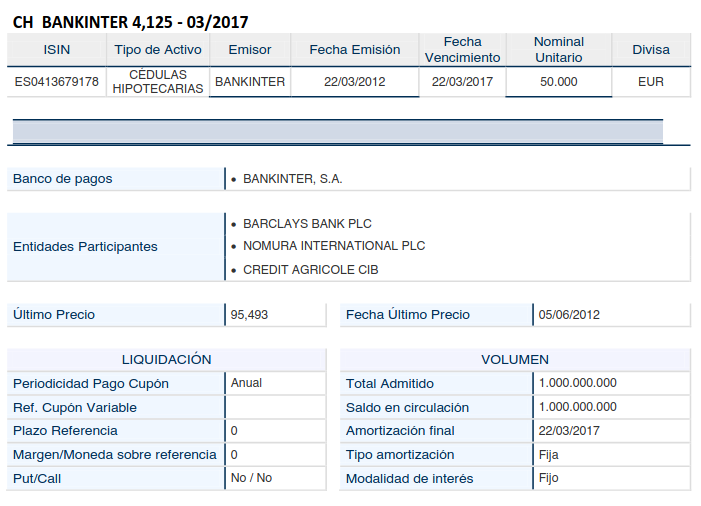
\includegraphics[width=0.9\textwidth]{../images/ej13.png}
    \caption{Cédulas Hipotecarias}
    \label{fig:cedulas}
\end{figure}

\begin{itemize}
    \item[a)] ¿Qué precio se pagó por cada Cédula Hipotecaria cuando se compró el 5/6/2012? \textbf{Sol: 48.170,30€}
    \item[b)] ¿Qué ecuación verifica la TIR con la que se contrataron estas Cédulas Hipotecarias el 5/6/2012? Comprueba que la TIR tiene un valor de 5,20\%.
    donde \(C\) es el cupón anual, \(F\) es el valor nominal, \(n\) es el número de años hasta el vencimiento, y \(TIR\) es la tasa interna de retorno.
    \item[c)] Sabiendo que el 5/6/2012 la duración de estas cédulas tenía un valor de 4,405537, ¿qué precio hubieran tenido las cédulas si la TIR se hubiera incrementado en 20 puntos básicos? \textbf{Sol: 47.766,87€} \textit{SIN RESOLVER}
\end{itemize}


\subsection*{Ejercicio 14}

La sociedad GADEB obtuvo financiación colocando en el mercado pagarés de empresa mediante una subasta competitiva. Estos pagarés tenían un nominal unitario de 6.000€ y vencimiento en 1 año. Después de anunciar la subasta en el mercado se recibieron las siguientes peticiones:

\begin{table}[H]
    \centering
    \begin{tabular}{|c|c|}
        \hline
        \textbf{Nominal (millones €)} & \textbf{Precio solicitado} \\ \hline
        20 & 95,975 \\ \hline
        30 & 95,885 \\ \hline
        35 & 94,975 \\ \hline
        25 & 94,555 \\ \hline
        10 & 94,375 \\ \hline
    \end{tabular}
\end{table}

Hoy, tres meses después de emitirse, estos pagarés se negocian en el mercado secundario mediante operaciones al contado al 4\% y también mediante operaciones con pacto de recompra a 15 días y al 3,5\%.

\begin{enumerate}[label=\textbf{\alph*)}]
    \item Resuelve la subasta sabiendo que la sociedad adjudicó un total de 100 millones y que para la adjudicación se usaron reglas similares a las aplicadas por el Tesoro Español. \textbf{Sol: medio: 95,385; marginal: 94,555}
    
    \item Calcula el tipo de interés marginal resultante de la subasta. \textbf{Sol: 5,7586\%}
    

    \item Si un inversor participó en la subasta solicitando pagarés a 94,975 y decide venderlos al contado hoy, ¿qué rentabilidad efectiva ha obtenido con ellos sabiendo que el intermediario en la operación de venta le cobra una comisión del 0,3\% sobre el efectivo de la venta? \textbf{Sol: 8\%}
    

    \item Calcula los precios que se fijan hoy en las operaciones con pacto de recompra y la rentabilidad efectiva que proporcionan este tipo de operaciones. \textbf{Sol: 5.846,53€; 5.855,05€; 3,6096\%}
    
\end{enumerate}





\subsection*{Ejercicio 15}

La empresa ALISUR posee en su cartera Letras del Tesoro por un nominal total de 60.000 euros. Estos valores fueron adquiridos en subasta al 7,75 \% de interés, con vencimiento a 92 días. Diez días después de la subasta la empresa debe realizar, en los 15 días posteriores, unos pagos por 39.290 euros, no disponiendo, en dicho momento, de liquidez para afrontarlos. El gerente de ALISUR decide solucionar el problema planteado a través de la venta de las letras, en la cantidad suficiente para hacer frente a los pagos. En estos momentos se puede conseguir para estos títulos un interés del 7,9335 \% en el mercado secundario. Una vez finalizado el período de pagos, la empresa volverá a adquirir las letras al 9,35 \% de interés. Los gastos totales de la operación de venta y compra se elevan al 2 por mil del nominal y se suponen pagaderos al final de la negociación simultánea.

Calcular el número de letras que debe vender ALISUR, el precio que habrá de pagar cuando decida comprarlas de nuevo y el coste que tiene asociado la operación de financiación diseñada. \textbf{Sol: 40 letras, 39.395,84€, 6,8\%}

\subsection*{Ejercicio 16}

El día 31/1/2017 un inversor contrató una operación simultánea sobre 100 obligaciones de la empresa ALALZA S.A. La operación simultánea estaba formada por las siguientes operaciones: compra al contado al 105,456 excupón y venta a plazo de 30 días (liquidación el 2/3/2017) al 4,504\% anual. Sabiendo que estas obligaciones tienen un nominal de 3.000€, pagan cupones anuales al 5\%, y vencen el 31/12/2030,

\begin{enumerate}
    \item[a)] ¿Cuánto pagó por cada obligación en la compra de la operación simultánea? \textbf{Sol: 3.176,42€}
    \item[b)] ¿Qué cantidad obtuvo por cada obligación en la venta de la operación simultánea? \textbf{Sol: 3.175,37€}
    \item[c)] Calcula la rentabilidad efectiva obtenida con esta operación simultánea \textbf{Sol: -0,40\%}
    \item[d)] En realidad, nuestro inversor esperaba, el 31/1/2017, que el precio de las obligaciones de la empresa ALALZA S.A. disminuyera en el mes siguiente; pensó que podría ser un buen negocio vender 100 obligaciones de esta clase para comprarlas 30 días después más baratas; y puesto que no disponía de dichas obligaciones, las adquirió temporalmente mediante la operación simultánea especificada en los apartados anteriores, para poder hacer la operación que había pensado. Si como había previsto nuestro inversor, el 2/3/2017 las obligaciones de ALALZA habían bajado de precio, cotizaban al 102,325 excupón. Calcula los beneficios o pérdidas que obtuvo nuestro inversor con la operación conjunta (operación simultánea + venta de las obligaciones el 31/1/17 y compra de las obligaciones el 2/3/2017). \textbf{Sol: 8.055,09€}
\end{enumerate}

\subsection*{Ejercicio 17}

Los fondos de inversión deben de tener una parte de su patrimonio invertida en activos muy líquidos para poder atender a los reembolsos de los partícipes; por ejemplo, en cuentas bancarias o en REPOS a un día. El 7/3/2017 los gestores del fondo INVERSIONES REUNIDAS contrataron una operación con pacto de recompra (REPO) sobre 1.500.000€ de nominal de Obligaciones del Estado con vencimiento el 31/1/2037 y cupón anual al 4,20\%. El REPO se contrató a 1 día y al -0,42\%. El precio de compra de las obligaciones al inicio del REPO (P1) se fijó como su precio de mercado con un recorte (haircut) del 5\%, de forma que P1=PMercado/(1+5\%). Sabiendo que el 7/3/2017 estas obligaciones cotizaban al 125,843 excupón, calcula:

\begin{enumerate}
    \item[a)] TIR con la que se estaban contratando las obligaciones en el mercado el 7/3/2017. \textbf{Sol: 2,529260\%}
    \item[b)] Cuantía pagada por el fondo al inicio de la operación REPO, 7/3/2017. \textbf{Sol: 1.803.510,57€}
    \item[c)] Cuantía que recibirá el fondo al final de la operación REPO, 8/3/2017. \textbf{Sol: 1.803.489,53€}
    \item[d)] ¿Cómo ha influido en la rentabilidad del fondo ésta operación? \textbf{Sol: Disminuye la rentabilidad}
\end{enumerate}


\section{Ejercicios Tema 2}

% \includepdf[pages=-,pagecommand={\thispagestyle{fancy}}]{Capitulos/Ejercicios_ISE_T2.pdf}

% \section{Diapositivas Tema 2}
% 
\includepdf[pages=-,pagecommand={\thispagestyle{fancy}}]{Capitulos/Tema2.pdf}


\newpage
% Referencias
\begin{thebibliography}{99}
\bibitem{Referencia1}
Ismael Sallami Moreno, \textbf{Estudiante del Doble Grado en Ingeniería Informática + ADE}, Universidad de Granada, 2025.
% \bibitem{Referencia2}
% Autor(es), \emph{Título del libro}, Editorial, año.

% \bibitem{Referencia3}
% Autor(es), \emph{Título del documento}, Nombre de la Conferencia, páginas, año.
\end{thebibliography}

\end{document}
